\section{Results}

%%%%%%%%%%%%%%%%%%%%%%%%%%%%%%%%%%%%%%%%%%%%%%%%%%%%%%%%%%%%%
%%  Optimal loading paths for parameter estimation  %%%%%%%%%

\subsection{Optimal \textit{in silico} loading paths for parameter estimation}

	The optimal loading paths for reproducing the response of dense collagenous soft tissues such as bovine pericardium and porcine aortic valve consist of 8 loading paths (Fig. \ref{fig:doptimality}C): 5 loading paths consisting of only inplane extensions (Fig. \ref{fig:doptimality}D), and 3 with the addition of the shear component. The increase in D-optimality is significantly less after three loading paths for the in-plane extensions (Fig. \ref{fig:doptimality}A). Same is true for the loading paths with shear. These three loading paths are the equibiaxial stress (Fig. \ref{fig:doptimality}B, Blue), and two uniaxial loading paths (Black, Green). The type of stress is consistent with the stress used for parameter estimation. The loading paths with shear simply iterates on these three loading paths by adding the shear component, we specified the maximum strain to be applied to be $0.2$. We consider this to be the minimal number of loading paths necessary for parameter estimation. In practice, it's better to add the intermediate inplane tension loading paths (Red, Orange) as a precaution, forming the full set of 8 loading paths (Fig. \ref{fig:doptimality}C). 
	
	
	The equi-biaxial stress loading path is the most important loading path. The D-optimality is $10^{-17}$ for the equi-biaxial loading path versus less than $10^{-300}$ (using \textit{Mathematica}'s extended precision) for other loading paths. The set of optimal loading paths will always contain the equi-biaxial stress loading path if the total number is odd, whereas it will always contain two loading paths just beside the equi-biaxial loading paths if it is even. The other loading paths complement the equi-biaxial loading path by spanning the range being searched. More details on the optimal loading path results are presented in appendix \ref{sec:optimalpaths}.
	
%-------------------	begin FIGURE 	-------------------%
\begin{figure}[hbtp]
\centering
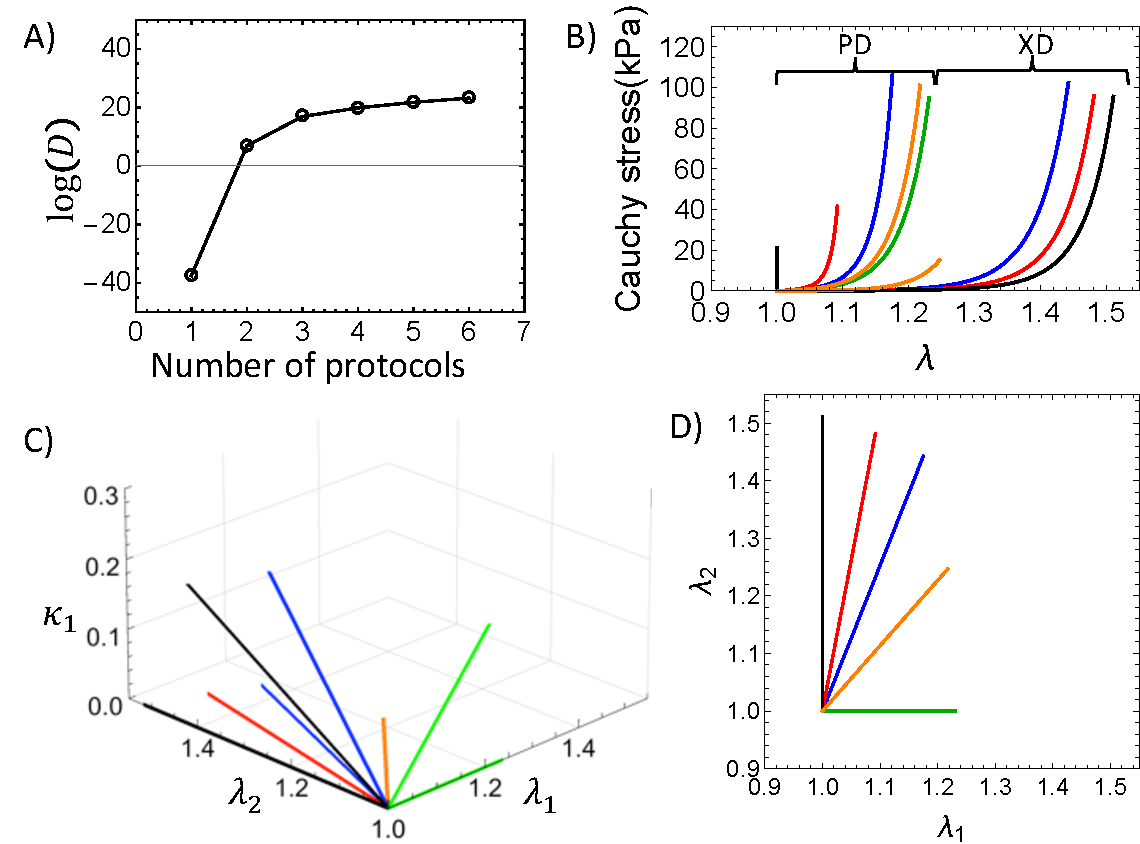
\includegraphics[width=5.5in]{Images/chapter5/doptimality}
\caption{A) The best D-optimality value for a given number of loading paths used to generate the data, which stops increasing significantly after three. B) The stress-strain curve of the optimal set of five loading paths with no shear. C) The full set of optimal loading paths including the shear component are shown. The same colored loading paths are built upon the corresponding D) planar stretch loading paths by adding a shear component. }
\label{fig:doptimality}
\end{figure} 
%-------------------	 end FIGURE 	-------------------%









%%%%%%%%%%%%%%%%%%%%%%%%%%%%%%%%%%%%%%%%%%%%%%%%%%%%%%%%%%%%%
%%  Parameter estimation and the quality of fit             %

\subsection{Parameter estimation and the quality of fit}

    The time taken for parameter estimation (5-10 seconds) is significantly lower in comparison to meso-scale structural approaches, such for the mitral valve \cite{zhang_meso_2016} (10-40 minutes) and exogenously crosslinked tissues \cite{zhang_modeling_2017}(30 min - 4 hours). In addition, we found that the model scaling method significantly improves the consistency of convergence. Parameters converges in approximately 40-60 iterations regardless of starting point, whereas it can vary between 40-120 iterations without using scaling. The additional iterations occur within the valley like region in the objective function surface (Fig. \ref{fig:objfunctionsurfaces}), where the gradient and thus the step size is very small. Of course, we found both methods to be essentially equivalent with a sufficiently good initial guess. We note that the model scaling method does not improve the correlations between the exponent parameters $b_1-b_{13}$ in $Q$. With that being said, the correlations between the exponent parameters $b_1-b_{13}$ are significantly better than the correlations between these exponents and modulus $c_0$ (Fig. \ref{fig:gvsecorrelation} and Appendix \ref{sec:parametercorrelation} Table \ref{tb:correlationE} \& \ref{tb:correlationG} vs. Table \ref{tb:ABcorrelation}), which is not much of a problem for parameter estimation. It is difficult to further improve the parameter correlation of $Q$ without changing the form of the model, but, for our purpose, this is already sufficient. 
    
    
    Qualitatively, $\Psi_{eff}$ (Eqn. \ref{eqn:finalexponentialmodelformscaled}) matches the response of collagenous soft tissues reproduced using the structural model (Eqn. \ref{eqn:fullcollagen}). It is able to follow all the characteristics of the response function (derivatives of the strain energy density function), including the symmetry with respect to shear (Fig. \ref{fig:modelfit}). The average $R^2$ is 0.958 (n = 6) for the bovine pericardium specimens tested. We found similar values for porcine aortic valve leaflets. The main improvements are in the uniaxial strain regions. 
%-------------------	begin FIGURE 	-------------------%
\begin{figure}[hptb]
\centering
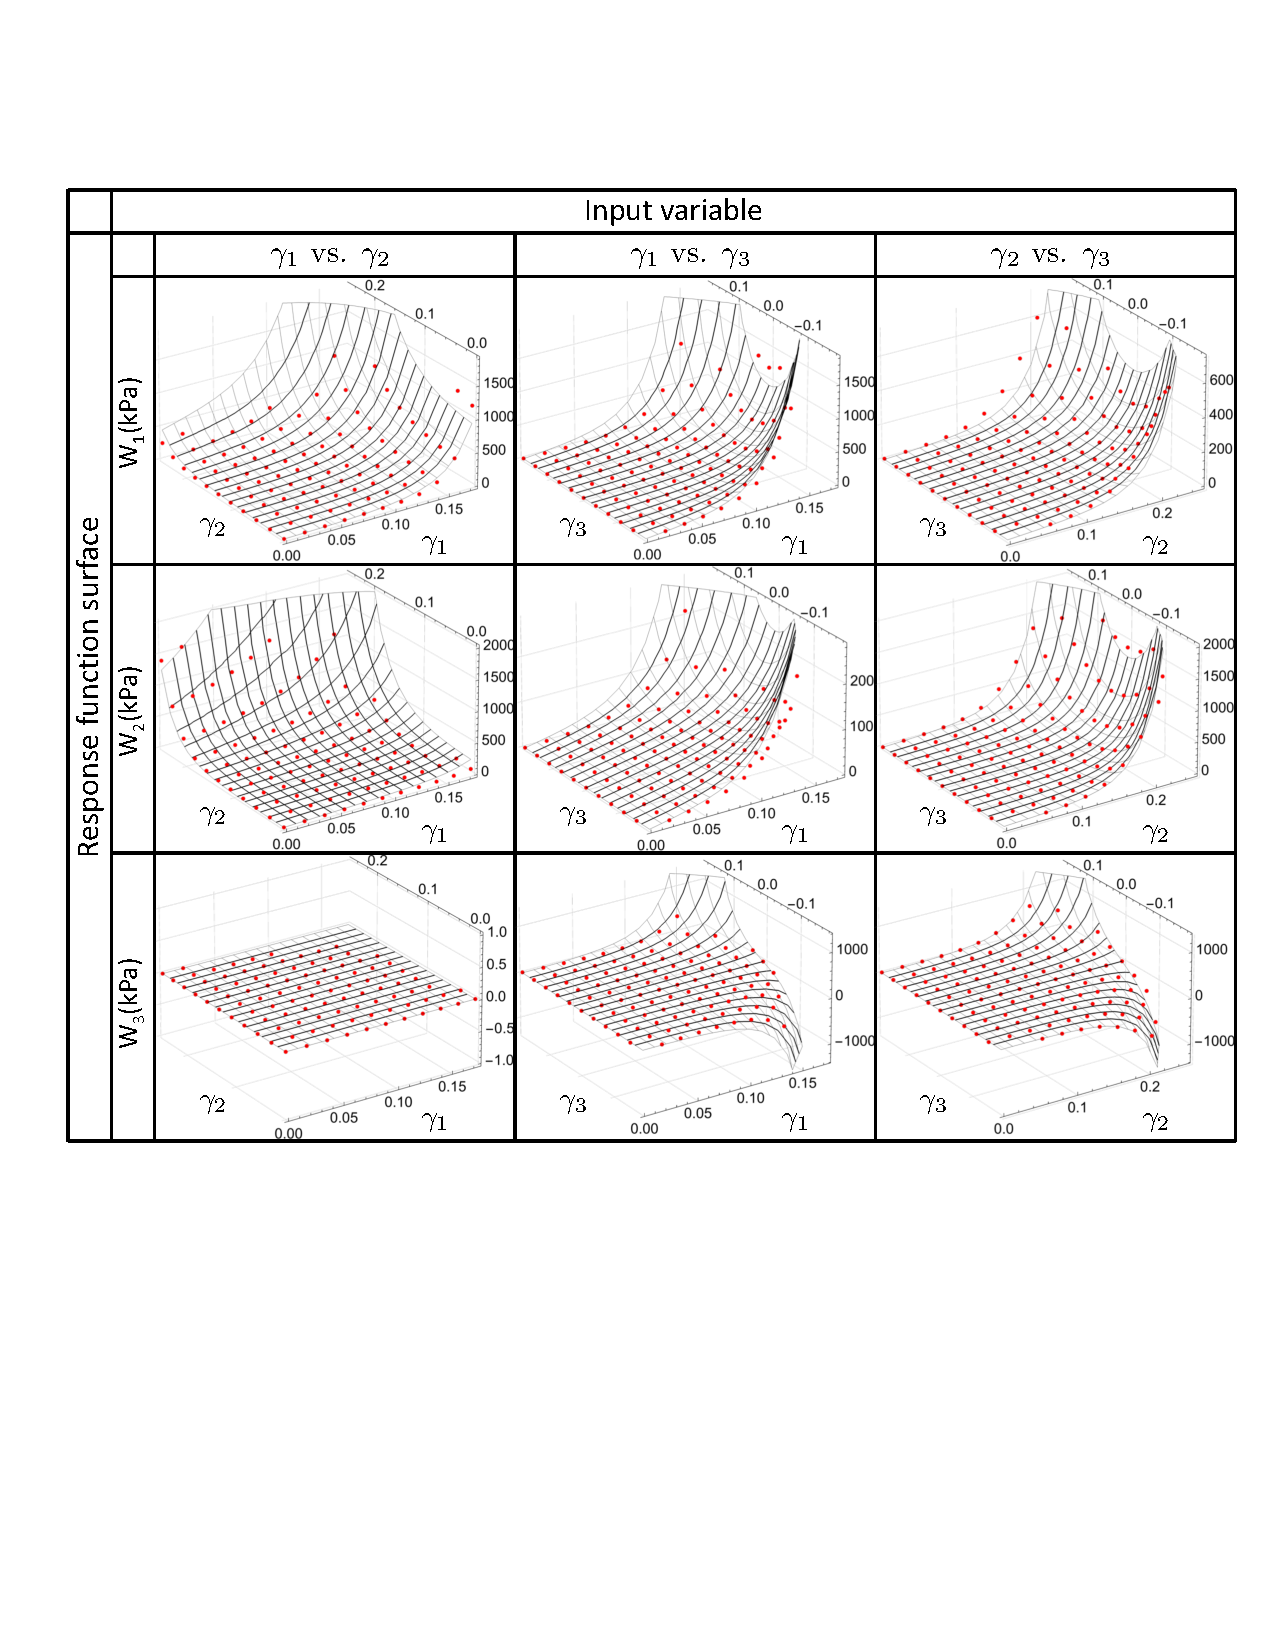
\includegraphics[width=\textwidth]{Images/chapter5/modelfit}
\caption{Parameter estimation results showing that $\Psi_{eff}$ is able to replicate the response function of the structural model (Eqn. \ref{eqn:objectivefunction}) (Top) $S_m = \partial\Psi/\dif E_m$, (Middle) $S_n = \partial\Psi/\dif E_n$, and (Bottom) $S_\phi = \partial\Psi/\dif E_\phi$ for each pair of Green Lagrange strain components.}
\label{fig:modelfit}
\end{figure} 
%-------------------	 end FIGURE 	-------------------%


    For a more detailed comparison, we replicated the result of Sun \textit{et al.} \cite{sun_biaxial_2003}. Similarly, we found that the generalized Fung model (Eqn. \ref{eqn:generalizedfungmodela}) fitted the five loading paths in the physiologic range very well (Fig. \ref{fig:fungphyfit}), but predicted the remaining unfitted loading paths poorly (Fig. \ref{fig:fungphypred}). When the non-physiologic loading paths are fit ((Fig. \ref{fig:fungphyfit})), the remaining protocols are still predicted poorly. However, we do note here that the generalized Fung model cannot fit the non-physiologic protocols very well, illustrating the limitation of the generalized Fung model at fitting the response of soft tissue in a wide range of deformations (Section \ref{sec:possibleforms}). 

%%%%%%%%%%%%%%%%%%%%%%%%%%%%%%%%%%%%%%%%%%%%%%%%%%%%%%%%%%%%
%-------------------	begin FIGURE 	-------------------%
\begin{figure}[hptb]
\centering
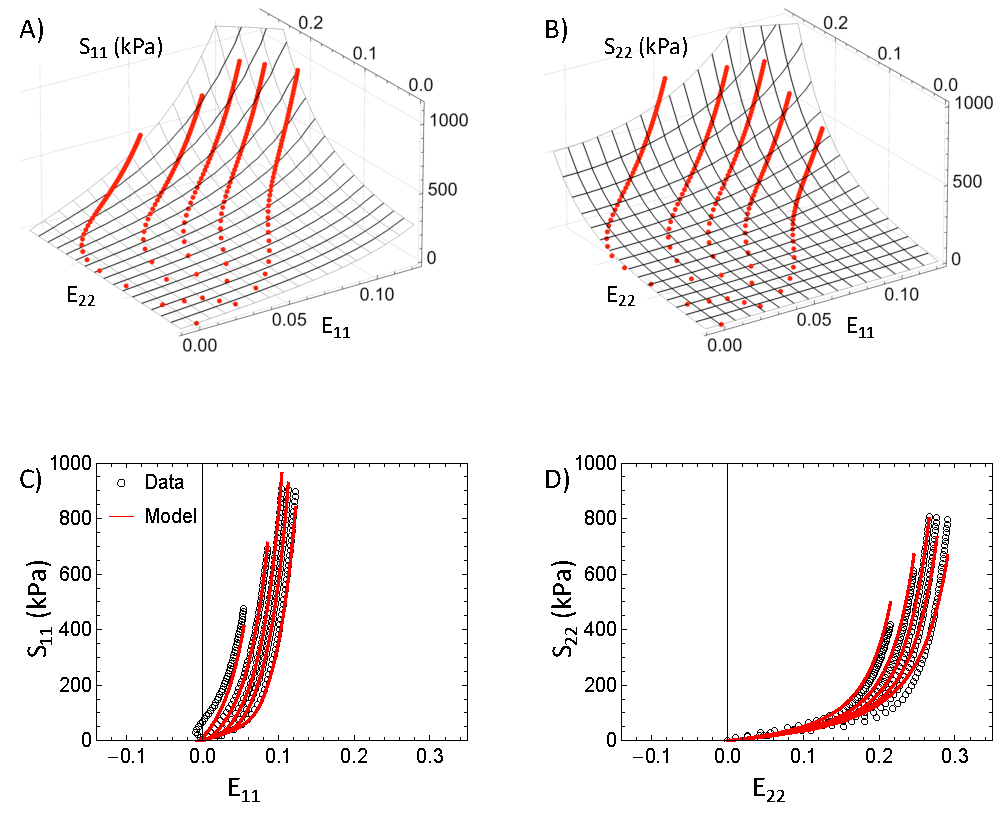
\includegraphics[width=\textwidth]{Images/chapter5/fungphyfit}
\caption{Reproducing the results of Sun \textit{et al.} \cite{sun_biaxial_2003} showing that the generalized Fung model is able to fit the loading paths in the physiologic range very well. A) The $S_{11}$ surface fitted to the data points. B) The $S_{22}$ surface fitted to the data points. C) Best fit of the $S_{11}$ component of the loading paths. D) Best fit of the $S_{22}$ component of the loading paths.}
\label{fig:fungphyfit}
\end{figure} 
%-------------------	 end FIGURE 	-------------------%
%%%%%%%%%%%%%%%%%%%%%%%%%%%%%%%%%%%%%%%%%%%%%%%%%%%%%%%%%%%%

%%%%%%%%%%%%%%%%%%%%%%%%%%%%%%%%%%%%%%%%%%%%%%%%%%%%%%%%%%%%
%-------------------	begin FIGURE 	-------------------%
\begin{figure}[hptb]
\centering
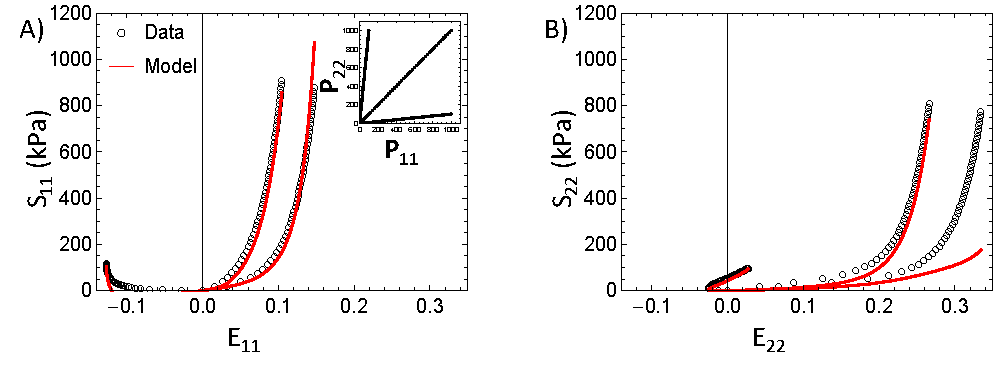
\includegraphics[width=\textwidth]{Images/chapter5/fungphypred}
\caption{Reproducing the results of Sun \textit{et al.} \cite{sun_biaxial_2003} showing the A) $S_{11}$ component and B) $S_{22}$ component of the remaining unfitted loading paths are predicted poorly from fit (Fig. \ref{fig:fungphyfit}). The inset in A shows the corresponding loading paths.}
\label{fig:fungphypred}
\end{figure} 
%-------------------	 end FIGURE 	-------------------%
%%%%%%%%%%%%%%%%%%%%%%%%%%%%%%%%%%%%%%%%%%%%%%%%%%%%%%%%%%%%


%%%%%%%%%%%%%%%%%%%%%%%%%%%%%%%%%%%%%%%%%%%%%%%%%%%%%%%%%%%%
%-------------------	begin FIGURE 	-------------------%
\begin{figure}[hptb]
\centering
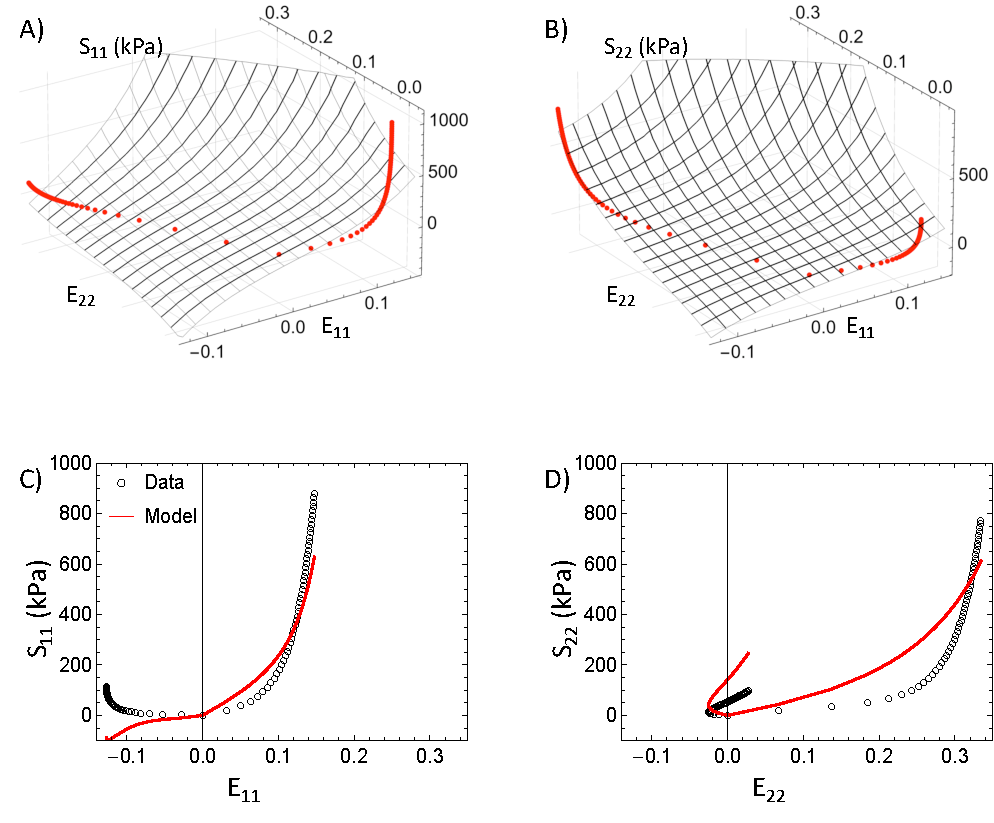
\includegraphics[width=\textwidth]{Images/chapter5/fungoutfit}
\caption{Reproducing the results of Sun \textit{et al.} \cite{sun_biaxial_2003} showing the best fit of the generalized Fung model to the loading paths in the non-physiologic range is poor. A) The $S_{11}$ surface fitted to the data points. B) The $S_{22}$ surface fitted to the data points. C) Best fit of the $S_{11}$ component of the loading paths. D) Best fit of the $S_{22}$ component of the loading paths.}
\label{fig:fungoutfit}
\end{figure} 
%-------------------	 end FIGURE 	-------------------%
%%%%%%%%%%%%%%%%%%%%%%%%%%%%%%%%%%%%%%%%%%%%%%%%%%%%%%%%%%%%

%%%%%%%%%%%%%%%%%%%%%%%%%%%%%%%%%%%%%%%%%%%%%%%%%%%%%%%%%%%%
%-------------------	begin FIGURE 	-------------------%
\begin{figure}[hptb]
\centering
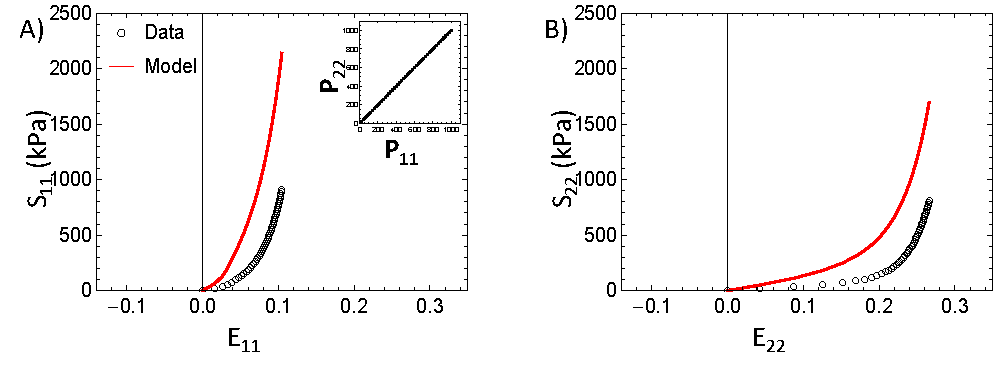
\includegraphics[width=\textwidth]{Images/chapter5/fungoutpred}
\caption{Reproducing the results of Sun \textit{et al.} \cite{sun_biaxial_2003} showing the A) $S_{11}$ component and B) $S_{22}$ component of the equi-biaxial stress loading path are predicted poorly from fit (Fig. \ref{fig:fungoutfit}). The inset in A shows the corresponding loading paths.}
\label{fig:fungoutpred}
\end{figure} 
%-------------------	 end FIGURE 	-------------------%
%%%%%%%%%%%%%%%%%%%%%%%%%%%%%%%%%%%%%%%%%%%%%%%%%%%%%%%%%%%%
    

	Using $\Psi_{eff}$ (Eqn. \ref{eqn:finalexponentialmodelformscaled}) (Fig. \ref{fig:effphyfit}) improves these results, but using non-optimal loading paths, such as based on Fung \textit{et al.}'s prestrained protocols \cite{fung_pseudoelasticity_1979}, lead to poor predictions for other loading paths (Fig. \ref{fig:effphypred}). Although not obvious at first, $\Psi_{eff}$ severely underestimates the response of the material in the low stress region. The D-optimality with two protocols in this prestrained range is only $1.35$, which improves to $1.98\times 10^4$ with six protocols. This pales in comparison to $9.7 \times 10^2$ for the two optimal protocols and $2.2 \times 10^7$ with three optimal protocols. When both $\Psi_{eff}$ and three optimal loading paths are utilized, we found that the loading paths are both fitted (Fig. \ref{fig:effoptfit}) and predicted very well (Fig. \ref{fig:effoptpred}). We also tested other non-optimal loading paths with modifications to the form of $\Psi_{eff}$ (Appendix \ref{sec:otherresults}). To briefly summarize these results, with an optimal set of loading paths, $\Psi_{eff}$ is able to fully reproduce the response of collagenous soft tissue for a wide range of deformation. However, without optimal loading paths, the form of $\Psi_{eff}$ can have unpredictable impact on the predicted response, even though the quality of fit is very similar. 


%%%%%%%%%%%%%%%%%%%%%%%%%%%%%%%%%%%%%%%%%%%%%%%%%%%%%%%%%%%%
%-------------------	begin FIGURE 	-------------------%
\begin{figure}[hptb]
\centering
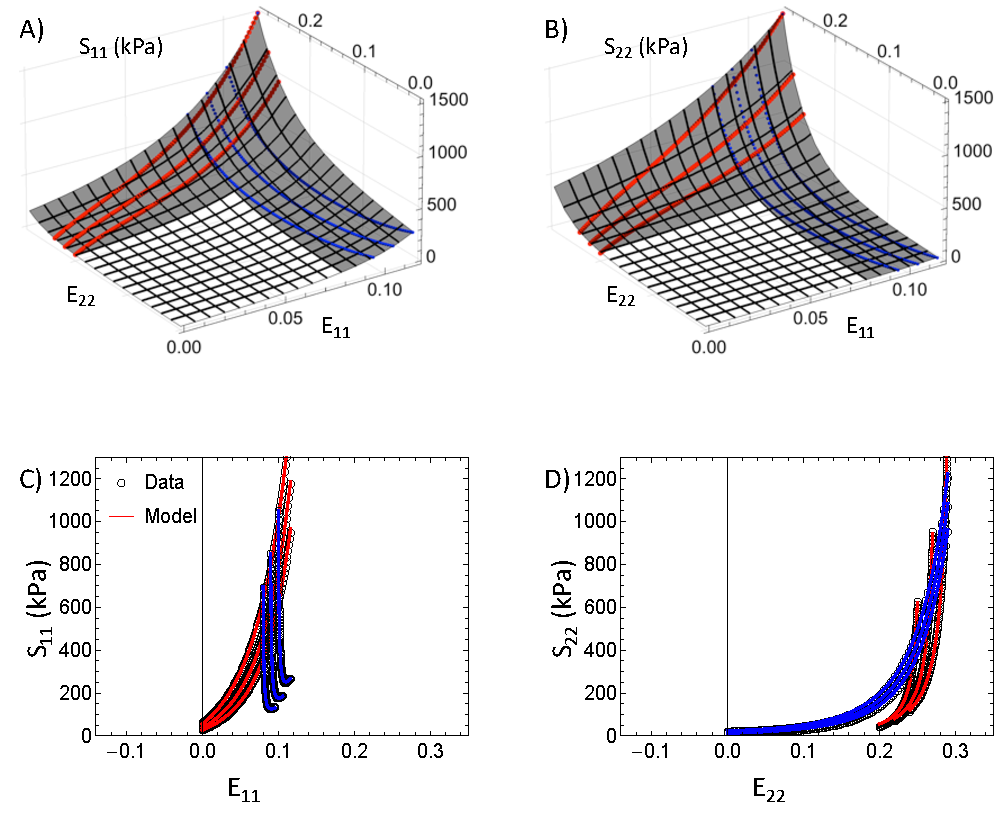
\includegraphics[width=\textwidth]{Images/chapter5/effphyfit}
\caption{The fit of $\Psi_{eff}$ to the prestrained loading paths is very good. A) The $S_{11}$ surface fitted to the data points. B) The $S_{22}$ surface fitted to the data points. C) Best fit of the $S_{11}$ component of the loading paths. D) Best fit of the $S_{22}$ component of the loading paths.}
\label{fig:effphyfit}
\end{figure} 
%-------------------	 end FIGURE 	-------------------%
%%%%%%%%%%%%%%%%%%%%%%%%%%%%%%%%%%%%%%%%%%%%%%%%%%%%%%%%%%%%

%%%%%%%%%%%%%%%%%%%%%%%%%%%%%%%%%%%%%%%%%%%%%%%%%%%%%%%%%%%%
%-------------------	begin FIGURE 	-------------------%
\begin{figure}[hptb]
\centering
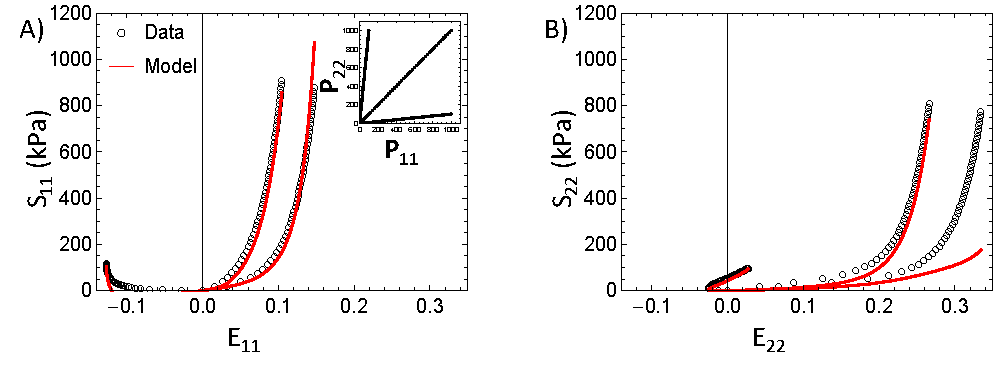
\includegraphics[width=\textwidth]{Images/chapter5/effphypred}
\caption{$\Psi_{eff}$ predicts the A) $S_{11}$ component and B) $S_{22}$ component of the unfitted loading paths very poorly even though the fit to the prestrained range is very good (Fig. \ref{fig:effphyfit}). The inset in A shows the corresponding loading paths.}
\label{fig:effphypred}
\end{figure} 
%-------------------	 end FIGURE 	-------------------%
%%%%%%%%%%%%%%%%%%%%%%%%%%%%%%%%%%%%%%%%%%%%%%%%%%%%%%%%%%%%


	

%%%%%%%%%%%%%%%%%%%%%%%%%%%%%%%%%%%%%%%%%%%%%%%%%%%%%%%%%%%%
%-------------------	begin FIGURE 	-------------------%
\begin{figure}[hptb]
\centering
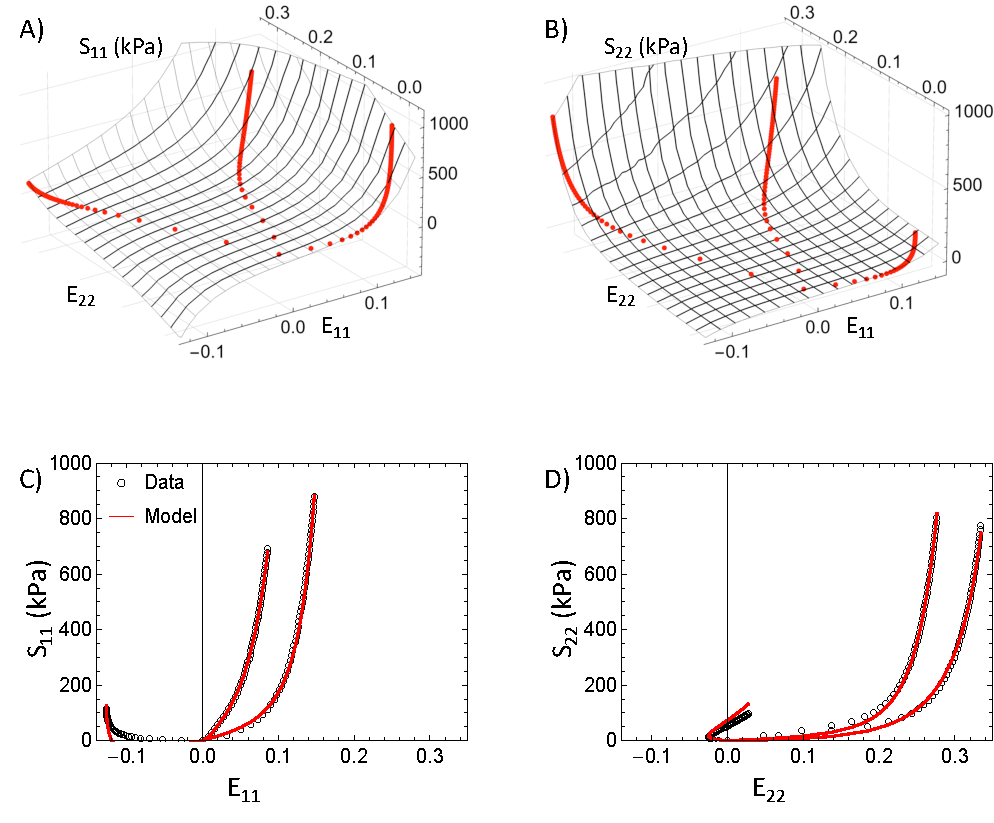
\includegraphics[width=\textwidth]{Images/chapter5/effoptfit}
\caption{$\Psi_{eff}$ fit optimal loading paths very well. A) The $S_{11}$ surface fitted to the data points. B) The $S_{22}$ surface fitted to the data points. C) Best fit of the $S_{11}$ component of the loading paths. D) Best fit of the $S_{22}$ component of the loading paths.}
\label{fig:effoptfit}
\end{figure} 
%-------------------	 end FIGURE 	-------------------%
%%%%%%%%%%%%%%%%%%%%%%%%%%%%%%%%%%%%%%%%%%%%%%%%%%%%%%%%%%%%

%%%%%%%%%%%%%%%%%%%%%%%%%%%%%%%%%%%%%%%%%%%%%%%%%%%%%%%%%%%%
%-------------------	begin FIGURE 	-------------------%
\begin{figure}[hptb]
\centering
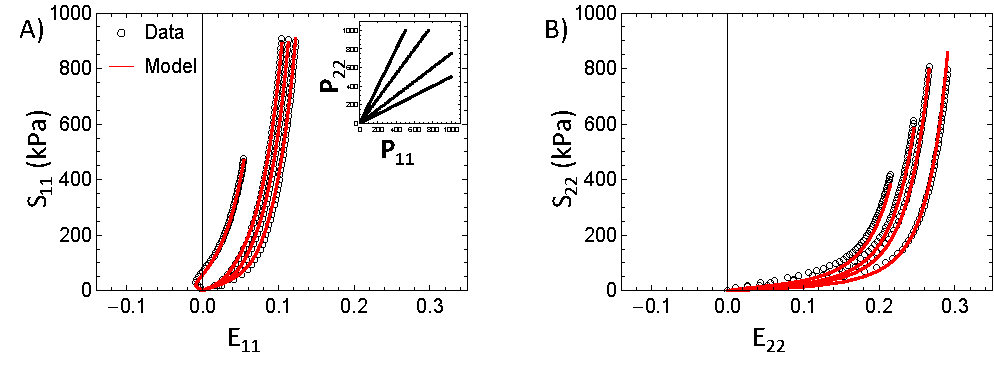
\includegraphics[width=\textwidth]{Images/chapter5/effoptpred}
\caption{Combining $\Psi_{eff}$ with optimal loading paths to predicts the A) $S_{11}$ component and B) $S_{22}$ component of the remaining unfitted loading paths very well from fit (Fig. \ref{fig:effoptfit}). The inset in B shows the corresponding loading predicted paths.}
\label{fig:effoptpred}
\end{figure} 
%-------------------	 end FIGURE 	-------------------%
%%%%%%%%%%%%%%%%%%%%%%%%%%%%%%%%%%%%%%%%%%%%%%%%%%%%%%%%%%%%





	



%%%%%%%%%%%%%%%%%%%%%%%%%%%%%%%%%%%%%%%%%%%%%%%%%%%%%%%%%%%%%
%%  Application to numerical simulations of BHVs under      %
%   quasistatic loading                                     %

\subsection{Numerical simulation of equibiaxial tension process and simulated bioprosthetic heart valve deformation}
	
    Planar biaxial test simulations were conducted to ensure that $\Psi_{eff}$ (Eqn. \ref{eqn:finalexponentialmodelformscaled}) and the elasticity tensor (Appendix \ref{sec:elasticitytensor}, Eqn. \ref{eqn:greenelasticityform}) were properly implemented in the finite element simulation framework.  We compared the computation time for both $\Psi_{eff}$ and Holzapfel-Gasser-Ogden model for biaxial simulation of bioprosthetic heart valve tissues and expectedly found no significant increase in computational cost. The total elapsed time for $\Psi_{eff}$ is 7.58 seconds in comparison to 6.40 seconds for the Holzapfel-Gasser-Ogden model, much faster than any micro-models can achieve.  

	Next we simulated tri-leaflet valves with model parameters derived from bovine pericardium, porcine aortic valve leaflet, and an idealized isotropic case. This is a simple demonstration of the use of the $\Psi_{eff}$ for the upscaling and homogenizing of micro-models. The model parameters for the bovine pericardium case were derived from the simplified structural model and model parameter of Aggarwal and Sacks \cite{aggarwal_inverse_2015}, and the resulting response matched very well qualitatively. Due to a lack of fiber mapping in the quasi-static simulation software used, some minor difference are still expected. We found no difficulty when simulating the pericardium, aortic, or isotropic valves. Suggesting that $\Psi_{eff}$ is quite robust numerically.
	
	
\begin{figure}
\centering
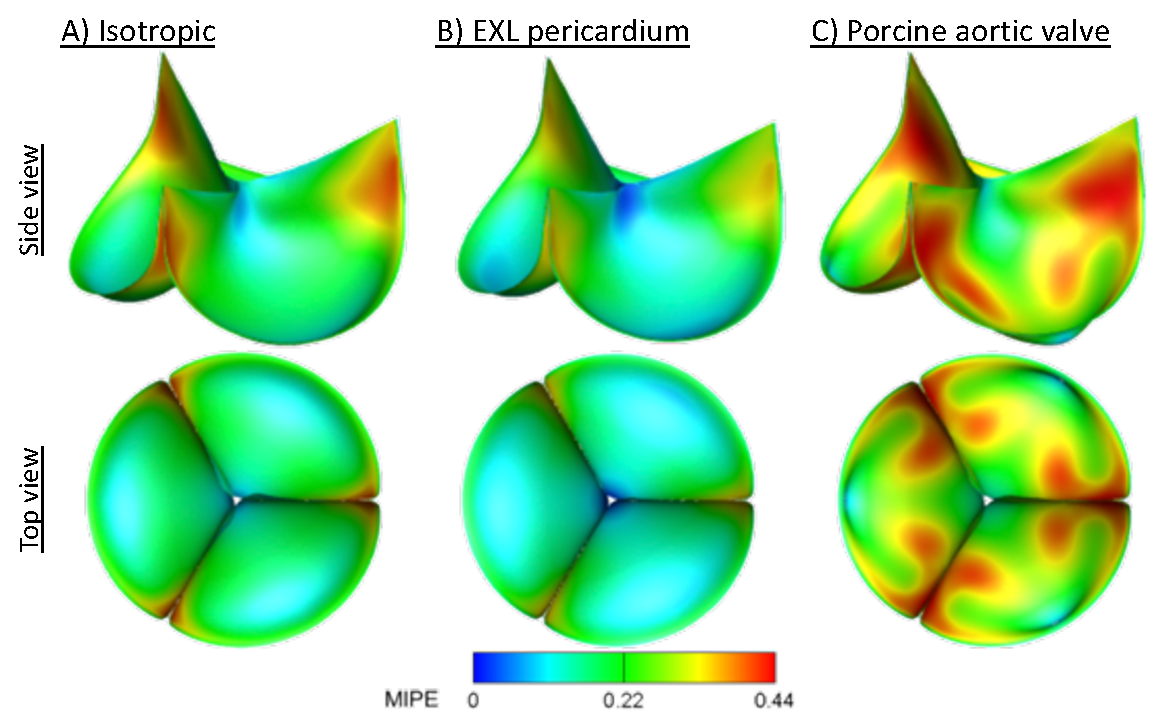
\includegraphics[width=\textwidth]{Images/chapter5/valvesimulations}
\caption{Simulations of intact tri-leaflet valves using A) the porcine aortic valve properties with an uniform fiber orientation distribution, B) exogenously cross-linked bovine pericardium properties with the most homogenous stress distribution, and C) the porcine aortic valve properties properties which results in a very heterogeneous stress distribution and the belly region caving in. The top row shows the side view of the valves at 80 mmHg and the bottom row shows the top-down view of the valves at the same transvalvular pressure.}
\label{fig:valvesimulations}
\end{figure}
    
    The material properties have significant effects on the mechanical behaviors of the leaflets (Fig. \ref{fig:valvesimulations}). The strain distributions within the leaflets were obtained for the pressure-loaded, fully-closed configurations of the valve, and then plotted with the maximum in plane Green-Lagrange strain (MIPE). When comparing the three different material, we can see that the native aortic valve properties result in significant heterogeneities in the deformation of the leaflets (Fig. \ref{fig:valvesimulations}C). Specifically, the belly region of the leaflets significantly protrudes out, increasing the load in the surrounding regions, especially near the commissures. This results in some stress concentrations that are not conducive to heart valve durability and health in general. The bovine pericardium valve (Fig. \ref{fig:valvesimulations}B) and the isotropic valve (Fig. \ref{fig:valvesimulations}A) on the other hand have significantly more homogeneous leaflet deformations, especially from the top-down view. Both of these undergo approximately the same deformation of 0.2 in MIPE. The largest difference between the two is near the commissure regions of the valve. Where the isotropic case is under significantly higher strain. Functionally, the material properties of the exogenously cross-linked bovine pericardium are the most suitable for heart valve leaflets, which distributes the stresses more evenly. 
    
    Much of the reasons behind these differences are likely to be due to the differences between the apparent mechanical properties \textit{in vivo} and the measured mechanical response in the laboratory setting. This is especially true for the aortic valve, which is extremely anisotropic with very high compliance in the radial direction of the leaflets. This difference is most likely due to the mismatch of referential configuration between the two states. Residual strain or residual stress has significant impact on the functional properties of the leaflets, specifically the apparent anisotropy and stiffness. Collagen fiber directions and varying regional properties can also have significant impact on the functional properties of the leaflets, and thus the results of the simulation. The valve leaflet shape, root geometry and properties, the arterial or ventricular geometry and loading conditions, can all be significant factors affecting the functions and stress distribution of the valve leaflets. Furthermore, how these factors affect the fluid dynamics of the valves is also an interesting question, suitable for further study. All in all, this is meant to be a demonstration and proof of concept for using $\Psi_{eff}$ to handle a wide range of soft tissue behaviors and anisotropy for the simulation of biological organs, in this case heart valves. Further and more detailed studies will be reserved for the future.  
  

    
    

